% ポストプロダクション段階で、エディターはカットやエフェクトなど様々な作業をしなくてはならない
In the post-production stage, an editor should do a lot of operations such as cutting scenes with mistakes, removing unexpected noise, applying audio and visual effects at appropriate timings, {\it etc}.
% それらの作業のために必要な情報は撮影時に発生するが、逐一ビデオと別途記録するのは面倒である
Most of information needed for the process, such as when an actor appeared in a scene, are shown during the shooting, however, we cannot note all of them with ordinary equipment.

\begin{figure}[htbp]
 \begin{center}
  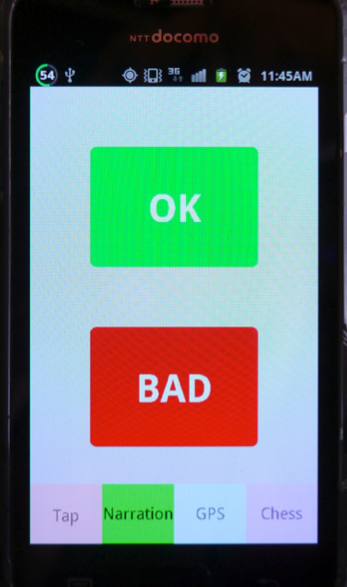
\includegraphics[height=70mm]{application_edit_app.png}
  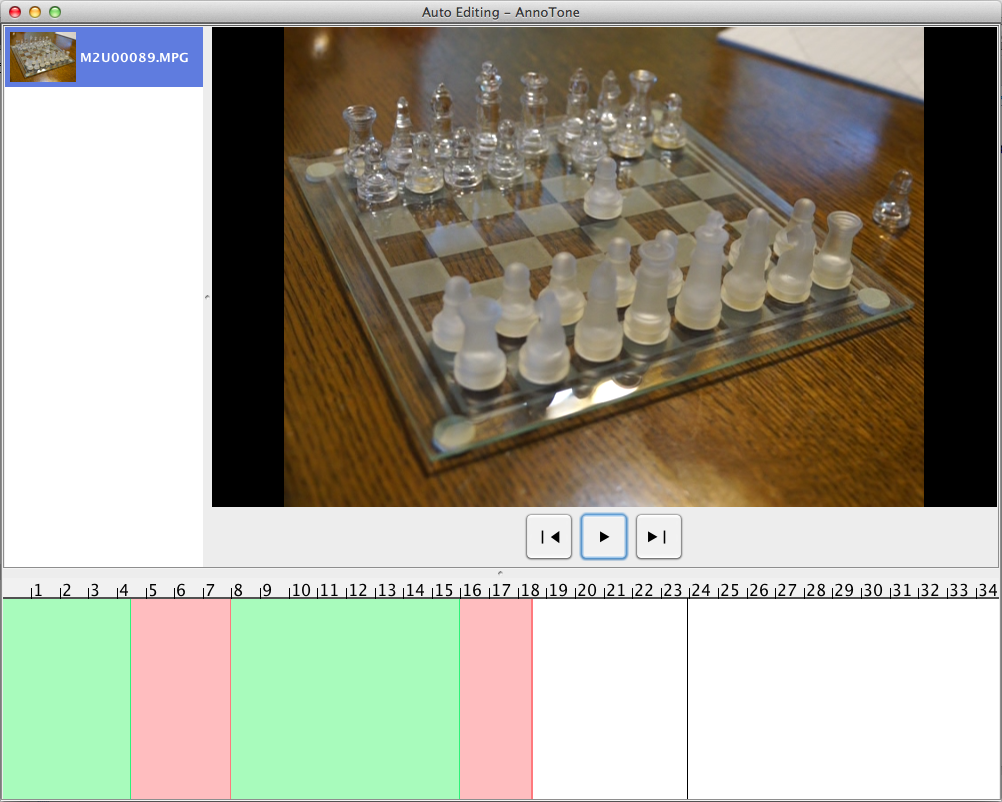
\includegraphics[height=70mm]{application_edit.png}
 \end{center}
 \caption{Left: The user interface of annotating application. Right: Automatic video cutting application.}
 \label{fig:appl_edit}
\end{figure}

% AnnoToneを使えば、そういう情報を録画中に埋め込んでおいて自動編集に使える
Using AnnoTone, we can embed that kind of information into a video in recording time, and conduct automatic editings after recording in accordance with the recorded annotations.
% 映像から失敗の部分を自動で切り取る、とても簡単なアプリケーションを作成した。
We created a very simple video editing application as a example of such usage, that automatically cut sections with mistakes off from a video.
% 使い方の説明
A camera person repeatedly taps one of the two buttons displayed on the interface (Figure \ref{fig:appl_edit} Left) of a smartphone during shooting a video to embed annotations that indicate whether the recent performance was good or not.
After the shooting, video editing application detects the annotations and divides the video into a series of sections at the annotated points.
Each section is marked ``OK'' or ``BAD'' based on the annotation that follows it, and sections marked ``BAD'' are cut off from the video.
% Figureの説明
The user interface of the application is shown in Figure \ref{fig:appl_edit} Right.
Timeline of the loaded video is displayed in the lower part of the interface, and each section is colored depends on how it is marked.
Red colored sections are marked ``BAD'', and they are automatically skipped when the user playback the video in the movie player above.
